For instance, the function
\begin{equation*}
    f(m) = m^e \bmod N = C, \quad (e, N) \mathrm{\; are \; public \; constants}, \quad m \; \mathrm{is \; secret}
\end{equation*}
is one-way function because it is easy to compute $C$ given $m$, but it is hard to compute $m$ given $C$.
The constants $(e, N)$ may be interpreted as an Alice's opened lock, whereas $m$ is a secret message from Bob.
Note that constants
\begin{itemize}
    \item $e$ is stands for encryption, public key
    \item $d$ is stands for decryption, private key
\end{itemize}
Now only one problem remains for the Alice -- is to define a pair of the keys $(e, d)$.
Alice knows that Bob encrypts his message $m$ as follows
\[
    m^e \bmod N = C
\]
To decrypt the message $C$ Alice must fetch a constant $d$ such that reverts the exponentiation of the
secret message $m$
\begin{eqnarray*}
    C^d = m \bmod N \\
    m^{ed} \bmod N = m \bmod N
\end{eqnarray*}
Firstly, Alice defines a public constant $N$ as a product of two large prime numbers $P, Q$
\[
    N = P \cdot Q
\]
so that it is hard to compute a factorization.

But how to fetch the secret constant $d$ to decrypt?
The Euler's totient theorem helps.
Given a number $N$ and its prime factorization $p_1^{e_1}\cdot p_2^{e_2} \cdots p_k^{e_k}$, the Euler's totient function
$\phi(N)$ is defined as
\[
    \phi(N) = (p_1^{e_1} - p_1^{e_1 - 1}) \cdot (p_2^{e_2} - p_2^{e_2 - 1}) \cdots (p_k^{e_k} - p_k^{e_k - 1})
\]
In particular, for the positive number $N$ such that its factorization is $p1 \cdot p2$, the $\phi(M)$ is
\[
    \phi(N) = (p_1 -1) \cdot (p_2 - 1)
\]
Euler's theorem relates the modular division and exponent as follows.
Given number $m$ then
\[
    m^{\phi(N)} = 1 \bmod N
\]
It means that reminder of division $m^{\phi(N)}$ by $N$ is always 1.
By the equality $1^K = 1$
\[
    m^{K \cdot \phi(N)} = 1 \bmod N
\]
If we multiply both parts by $M$, we get
\[
    m \cdot m^{K \cdot \phi(N)} = m^{K \cdot \phi(N) + 1} = m \bmod N
\]
It follows that Alice is able to define the secret $d$ as follows
\begin{gather*}
    e \cdot d = K \cdot \phi(N) + 1\\
    d = \frac{K \cdot \phi(N) + 1}{e}\\
\end{gather*}
The following image demonstrates the concept of RSA approach
\begin{figure}[H]
    \centering
    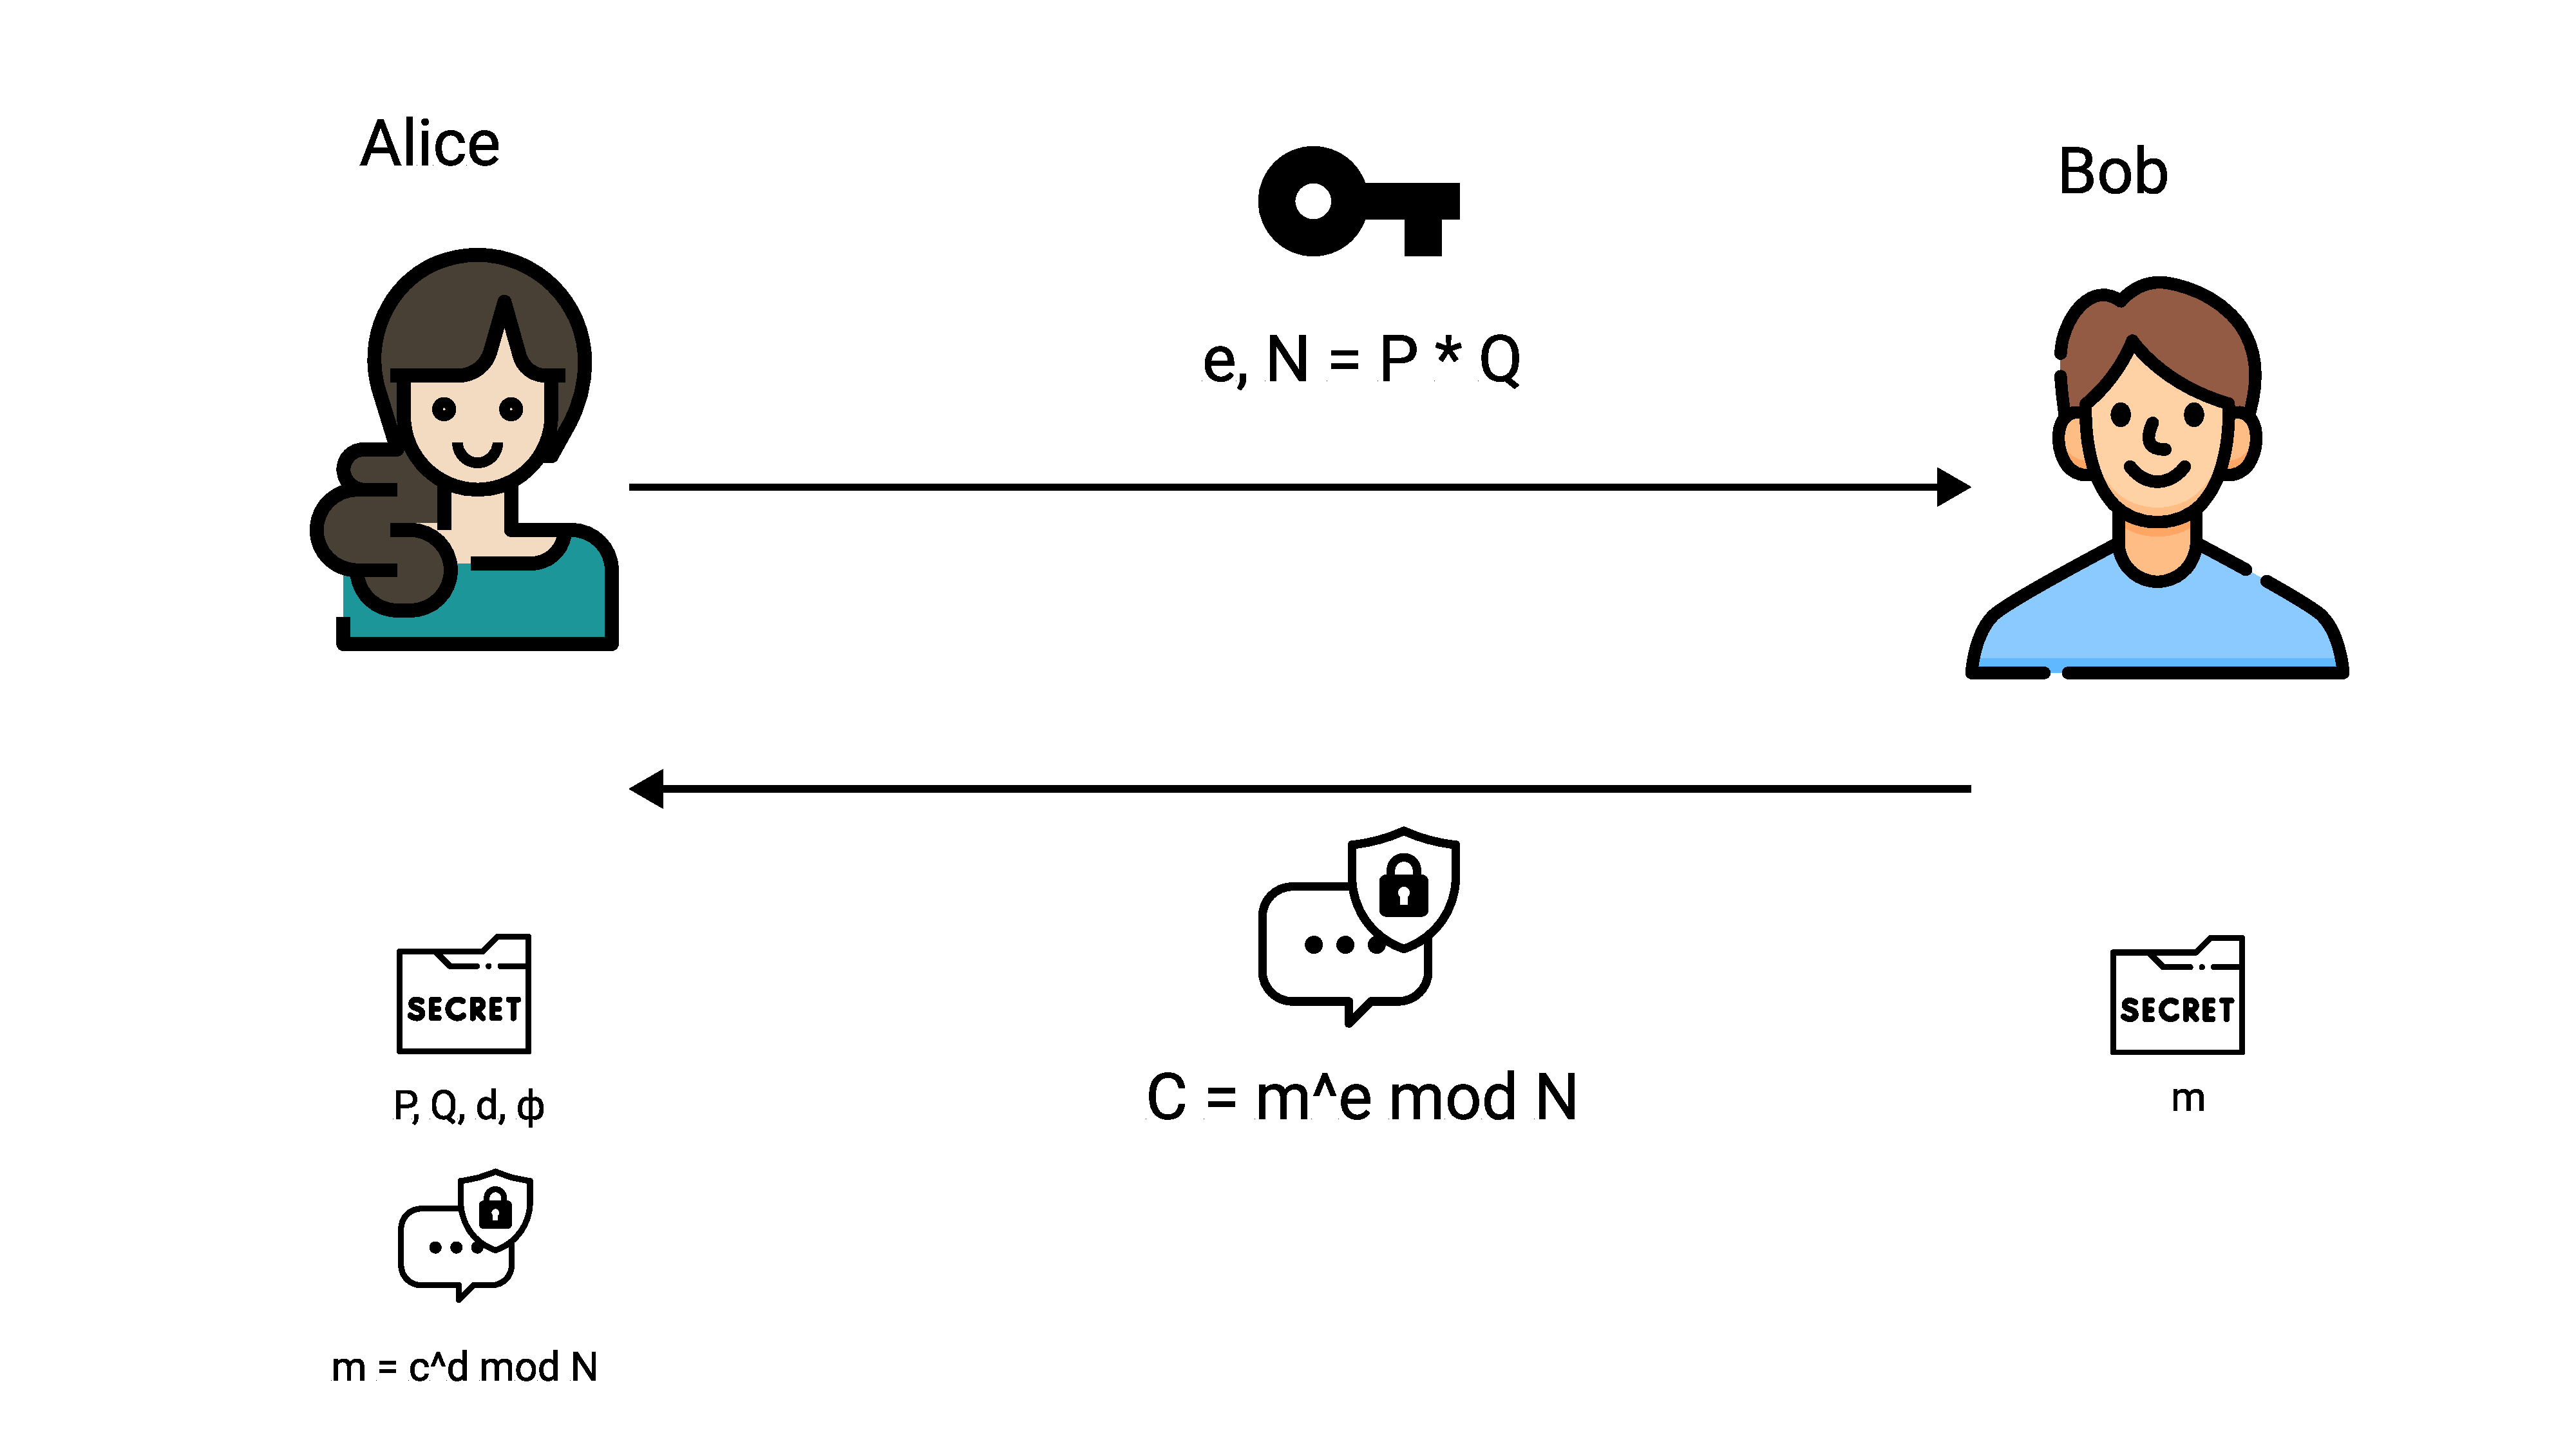
\includegraphics[width=1\textwidth]{./img/RSA}
    ~\caption{RSA algorithm concept diagram.}\label{fig:figure8}
\end{figure}
To summarize, the process by the steps is as follows
\begin{itemize}
    \item Alice defines the large secret prime numbers $P, \; Q$.
    \item Alice computes $N = P \cdot Q$ and $\phi = (P-1)(Q-1)$
    \item Alice chooses an integer $e$, $1<e< \phi$ such that $\gcd(e, \phi) = 1$.
    \item Alice computes secret exponent $d$, $1<d< \phi$ such that $ed \equiv 1 \bmod \phi$.
    \item Alice shares public key $(N,e)$ with Bob and keeps private key $(d, p, q)$ is secret.
    \item Bob defines the message $m$, encrypts it as $C = m^{e} \bmod N$.
    \item Bob sends $C$ to Alice.
    \item Alice decrypts $C$ using her secret $d$, so she gets $m$
    \[
        m = C^d \bmod N
    \]
\end{itemize}
Security of the RSA approach is based on the complexity of fundamental problem of prime factorization,
which takes decades to solve having enough large number.
